% !TEX TS-program = pdflatexmk
\documentclass[11pt,a4paper]{article}

\usepackage[english]{babel}
\usepackage[T1]{fontenc}
\usepackage{graphicx}
\usepackage[pdftex]{hyperref}
\hypersetup{
breaklinks=true,
pdfborder={0 0 0},
pdfstartview={FitH},
pdfpagemode={UseOutlines},
pdftitle={An adaptive cache server written in F\#},
pdfauthor={Filippo Sironi, Matteo Villa},
pdfsubject={Argomenti Avanzati di Ingegneria del Software},
pdfkeywords={F\#,.NET,Aware,Adaptive,Cache,Client/Server}
}
\usepackage{indentfirst}
\usepackage[applemac]{inputenc}
\usepackage{listings}
\lstset{basicstyle=\ttfamily,showstringspaces=false,captionpos=b,abovecaptionskip=1.5em}
\usepackage{url}

\begin{document}

\thispagestyle{empty}

\begin{center}
{\huge Politecnico di Milano}
\end{center}

\begin{center}
{\huge Argomenti Avanzati di Ingegneria del Software}
\end{center}

\vskip 8cm

\begin{center}
{\huge An adaptive cache server written in F\#}\\
\url{http://code.google.com/p/adaptive-cache-server/}
\end{center}

\vskip 2cm

\begin{center}
\begin{tabular}{ll}
{\large Filippo Sironi} & {\large 734456}\\
{\large Matteo Villa} & {\large 735064}\\
\end{tabular}
\end{center}

\vskip 5.5cm

\begin{center}
{\large 2009-2010}
\end{center}

\newpage

\section{Introduction}
\label{section:introduction}
Aim of this project is to explore the support that a given programming language and, if available, the underlying framework can provide in order to build an aware and adaptive software system.
While adaptation can be achieved through primitive constructs (such as an \emph{if} or \emph{case} chain that selects the desired behavior), our goal is to rely on a more powerful level of abstraction and higher level constructs among the ones offered by the platform.

The programming language adopted for this project is F\#, a multi-paradigm programming language leveraging the .NET framework.

\section{The F\# programming language and the .NET framework}
\label{section:platform}
The F\# project began in 2002 when Don Syme and others at Microsoft Research decided to propose the adoption of a functional programming language based on \emph{ML} for the .NET framework. Its first major pre-release was in 2005.

F\# is a statically strong typed programming language that supports many different paradigms. It shares a core language with the OCaml (Objective Caml) programming language, and in some ways it can be considered an ``OCaml for .NET''. F\# would not exist without OCaml, which in turn comes from the ML family of programming languages, which dates back to 1974. F\# also draws from the Haskell programming languages and other functional programming languages such as Erlang.

Despite being a functional programming language and being similar to OCaml and Haskell, we can say that F\# is a whole other kind of programming language. In fact, F\# can leverage the full power of .NET that allows the natural adoption of both the imperative and the object-oriented (OO) paradigms; moreover, F\# allows the exploitation of advanced constructs such as sequence expressions and workflows which are inspired by Haskell's monads. In addition to this, F\# also provides a missing link between compiled and the so called dynamic programming languages, combining the idioms and programming styles typical of dynamic programming languages with the performance and robustness of a compiled programming language.

Functional programming is booming at a point that some common functional programming constructs have been integrated into mainstream programming languages such as C\#, Python, Ruby, and more recently, Java.

\section{An adaptive cache server written in F\#}
\label{section:work}
The software system to build for this project is a cache server. As a basic behavior it simply offers a caching service, speeding up the retrieval of information generated on other machines. The type of items to store in the cache can be resources of any kind. The server exposes some simple primitives, such as \texttt{search(key)}, \texttt{store(value)}, and \texttt{remove(key)}. The cache server must be aware and adaptive.

The cache server implemented for this project leverages awareness and adaption in different contexts. In fact, it provides adaptation in accordance with the memory context, the logging context, and the network context.

\subsection{Memory context}
\label{section:work:memory-context}
The implemented cache server supports theoretically an infinite number of memory contexts which are partition in two major contexts. The first is called \emph{high memory context} while the second is \emph{low memory context}.

When the \emph{high memory context} is active the cache server is allowed to use an infinite amount of virtual memory and the sole memory limitation is given by the total amount of virtual memory the machine can address. This means every cache line is ``volatile'' in the sense that it is only resident within the volatile memory.

On the other hand, when the \emph{low memory context} is active there can be many different situations. The low memory context is coupled with a parameter indicating the upper bound of volatile memory the cache server can use to store cache lines. Once the bound is reached the cache server starts using the non-volatile memory.

\subsection{Logging context}
\label{section:work:logging-context}
Many different software systems support many different levels of logging. Usually the logging level is selected when the software system is started and cannot be changed at run-time. A peculiarity of aware and adaptive software systems is the capability of changing the way they operate without any down-time: therefore, the cache server here implemented has indeed the ability to change the amount of messages to be logged during its execution. It supports three different logging levels:
\begin{itemize}
\item \emph{error}, only error messages are logged;
\item \emph{warning}, warning and error messages are logged;
\item \emph{information}, (verbose context) logs information, warning, and error messages.
\end{itemize}

\subsection{Network context}
\label{section:work:network-context}
The last adaptation capability implemented is that regarding the network context. The cache server supports the ability to change the protocol used for the client/server communication while the system is running without any interruption.

\subsection{Implementation}
\label{section:work:implementation}
The cache server is logically partitioned in five different modules, as shown in Figure \ref{figure:modules}.

\begin{figure}
\begin{center}
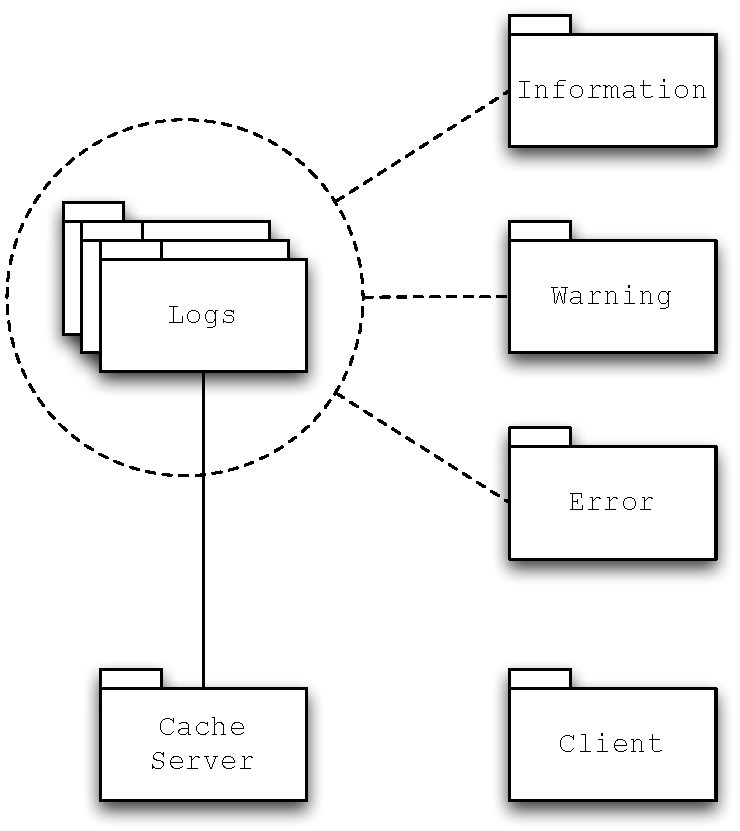
\includegraphics[width=0.75\textwidth]{figures/Modules.pdf}
\caption{Modules}
\label{figure:modules}
\end{center}
\end{figure}

The \emph{client} module contains all the code related to the client used to interact with the cache server; the \emph{cache server} module contains the code related to the server itself; while the three modules \emph{error}, \emph{warning}, and \emph{information} contain the code used to handled the three logging levels. Further explanations about this partitioning will be given later.

The client is a simple interactive application that has been developed making an extensive use of the functional programming paradigm. Its mutable state is concentrated in a set of mutable values which are used to handle the hot-swap of a network protocol, hence the change of the network context, in favor of another one. The application' s configuration is read, once the application is started, from an XML configuration file.  An example XML configuration file is shown in Listing \ref{listing:client-configuration}.

\begin{lstlisting}[language=XML,caption=Client XML configuration file,label=listing:client-configuration,float]
<configuration>
  <appSettings>
    <add key="IP-Address" value="127.0.0.1"/>
    <add key="TCP-Port" value="1234"/>
    <add key="Protocols" value="protocols.xml"/>
    <add key="Default-Protocol" value="0"/>
  </appSettings>
</configuration>
\end{lstlisting}

The cache server is made up of different components organized in different sub-modules as Figure \ref{figure:cache-server-modules} shows.

\begin{figure}
\begin{center}
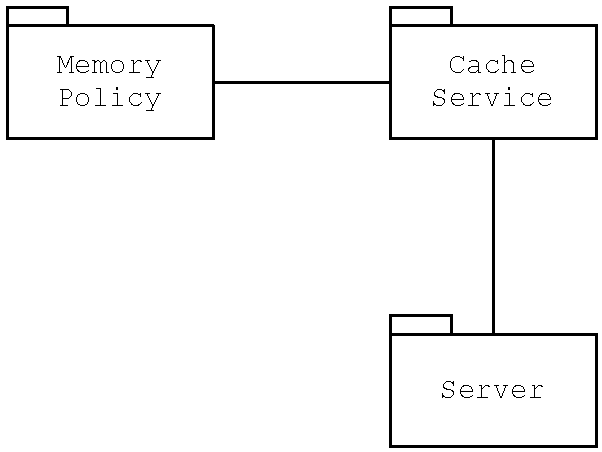
\includegraphics[width=0.65\textwidth]{figures/Cache-Server-Modules.pdf}
\caption{Cache server modules}
\label{figure:cache-server-modules}
\end{center}
\end{figure}

The \emph{server} module contains an interactive application whose execution cycle is split in two asynchronous tasks (threads). One of the task maintains an instance to the cache service while the other handles network communications and accesses the cache service running within the other task. The cache service is contained in the \emph{cache service} module. Finally, the \emph{memory policy} module contains the code that handles the different memory contexts. Just like the client, the cache server loads its initial configuration from an XML configuration file. An example XML configuration file is shown in Listing \ref{listing:cache-server-configuration}.

\begin{lstlisting}[language=XML,caption=Cache server XML configuration file,label=listing:cache-server-configuration,float]
<configuration>
  <appSettings>
    <add key="Server-Log-DLL"
         value="warning.dll"/>
    <add key="IP-Address"
         value="127.0.0.1"/>
    <add key="TCP-Port"
         value="1234"/>
    <add key="Protocols"
         value="protocols.xml"/>
    <add key="Default-Protocol"
         value="0"/>
    <add key="Console-Log"
         value="AdaptiveServerAdminConsole"/>
    <add key="Cache-Log"
         value="AdaptiveCacheService"/>
    <add key="Server-Log"
         value="AdaptiveServer"/>
  </appSettings>
</configuration>
\end{lstlisting}

\section{Involved abstractions and constructs}
\label{section:functionalities}
To achieve some level of adaptability, the implemented cache server tries to exploit different general purpose constructs provided by the language and the underlying platform themselves without relaying on an ad-hoc framework to manage contexts mainly because such a framework doesn't exist yet.

Having identified three different areas in which awareness and adaptation are useful and hence involved, the next step is to propose adopt a suitable adaptation method. Even if F\# and .NET are not supported by an ad-hoc framework for adaptation, they are a couple made up of a flexible programming language supporting many different programming paradigms and a powerful framework.

In this project three methods to provide adaptation as been exploited, namely they are:
\begin{itemize}
\item \emph{generic programming}, this computer programming style dates back to 1980s, however, it is a widely adopted techniques in both mainstream programming languages (\emph{i.e.,} C++, C\#, Java, and so on\ldots) and functional programming languages such as ``MLs'', Haskell, and Scala. F\# support of generics is built on top of .NET support;
\item \emph{reflective programming}, which is a computer meta-programming technique allowing software components to change their inner operations and structures modifying their behavior. Once again, F\# support of reflection depends on .NET;
\item \emph{pattern matching}, that is functionality common to many functional programming languages, F\# boosts its potential to an extent that allows adaptation.
\end{itemize}

\subsection{Generic programming}
\label{section:functionalities:generics}
Generic programming and \emph{generics} have been exploited in order to allow the cache server to adapt its behavior upon changes in the memory context. More precisely, two different memory policies to manage the high memory context and the low memory context have been implemented in two different function objects, the first is called \texttt{HighMemoryPolicy} while the latter is called \texttt{LowMemoryPolicy}, both of them are implemented within the memory policy module and inherit their public interface from \texttt{MemoryPolicy} (which is an abstract data type).

Whenever a memory context change occurs, the context controller sends a message to the cache service advising it to change the way it is operating. Take a more in depth look, a new memory policy is instantiated and it is used to substitute the active one. The instantiation of a new memory policy is demanded to a factory object which hides complexity to the software system developer. It is important to observe that this substitution is managed by the cache service in a completely transparent fashion since it imposes no lock on the software system since the main control loop of the cache service exploits two important functional programming functionalities: \emph{non-mutable values} and  \emph{recursion} (which is optimized away by the compiler through tail-recursion optimization).

Figure \ref{figure:memory-policies} shows the abstract data types tree.

\begin{figure}
\begin{center}
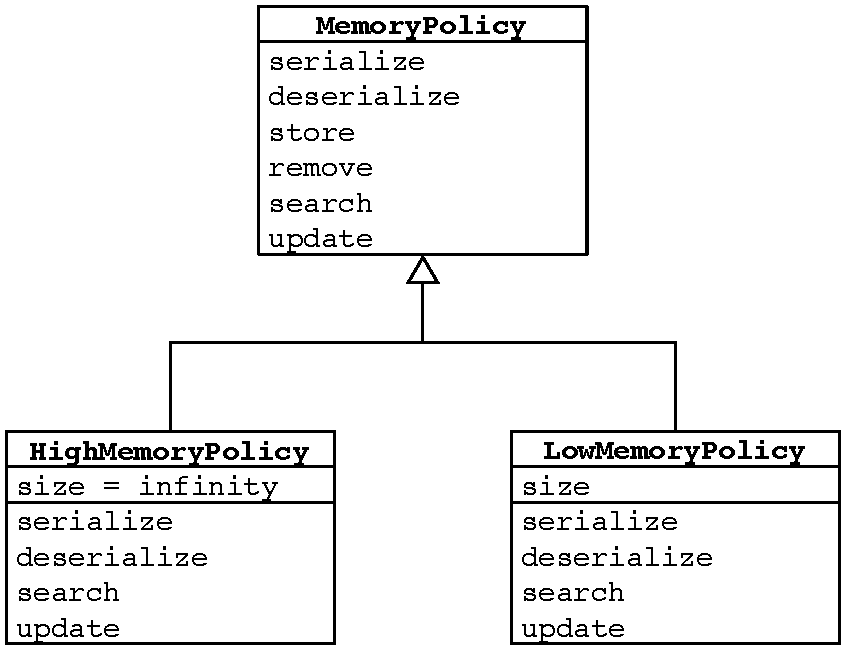
\includegraphics[width=0.85\textwidth]{figures/Memory-Policies.pdf}
\caption{Memory policies}
\label{figure:memory-policies}
\end{center}
\end{figure}

\subsection{Reflective programming}
\label{section:functionalities:reflection}
Reflective programming has been used to implement adaptation capabilities regarding the logging context. As discussed in Section \ref{section:work:implementation}, in addition to the ``common'' client and cache server modules this project contains three additional modules and all of them are recognized as a log module.

These three additional modules, information, warning, and error are built separately and encapsulated in three different \emph{dynamic-link libraries} (DLLs). These three DLLs export the same names, this characteristic proved to be fundamental for implementing adaptation.

The fact that these DLLs export the same names allows the cache server to hot-swap one in favor of another one and transparently load functions from the currently addressed library. The ability to dynamically load a function from a module enclosed within an external library and hence dynamically dispatch requests is a feature of the reflective sub-system built within .NET which grants the ability to fully inspect a .NET assembly.

In contrast with the approach chosen for the memory context adaptation process, which makes an extensive use of generic programming, generics, and an hierarchy of abstract data types, the approach adopted in conjunction with reflection is ``purely'' functional in the sense that it makes use of functions only without declaring abstract data types.

\subsection{Pattern matching}
\label{section:functionalities:pattern-matching}
Many times in computer programming data structures and their values needs to be examined and tested against one or more conditions. When these conditions are met, certain computations and transformations are triggered or particular actions are performed. To accomplish these types of operations in F\#, it is possible to use ``the good old'' \emph{if} chains; however, pattern matching, that is a quite common construct in functional programming languages, offers greater power and flexibility, and goes well beyond more primitive constructs.

Usually, the pattern matching mechanisms is completely static (\emph{i.e.,} possible matches are fixed at compile time and do not change during the execution of the program). F\# allows pattern to ``come alive'' so that it is possible to control and change them during the execution. This derived construct is known as \emph{active patterns}.

This project makes an extensive use of active patterns to implement network context adaptation; the adaptation process change the way active patterns parse and decompose both network and local messages ``on-the-fly'' while the software system is running. At the very base of active patterns there are a ``banana clipped function'' (that is not a regular function that can be used during the normal execution of a program but an ad-hoc function the F\# compiler is instructed to use only with active patterns) and a regular expression. Based on the the regular expression the active pattern function decomposed the input message in different ways so that it is simpler to bound values and analyze them.

Regular expressions used to guide the active pattern function are loaded from an XML file, Listing \ref{listing:protocols} shows an example.

\begin{lstlisting}[language=XML,caption=Protocols XML file,label=listing:protocols,float]
<?xml version="1.0" encoding="utf-8" ?>
<protocols>
  <protocol id="0">
    <store command="store: ">
      ^(store:)(\s+)(.+)$
    </store>
    <remove command="remove: ">
      ^(remove:)(\s+)(\d+)$
    </remove>
    <search command="search: ">
      ^(search:)(\s+)(\d+)$
    </search>
    <key command="key: ">
      ^(key:)(\s+)(\d+)$
    </key>
    <value command="value: ">
      ^(value:)(\s+)(.+)$
    </value>
    <error command="error: ">
      ^(error:)(\s+)(.+)
    </error>
  </protocol>
</protocols>
\end{lstlisting}

Since the protocol at the very base of both network and local communications is fundamental to allow the clients and the cache server to talk, the adaptive capabilities implemented by active patterns is used not only within the cache server but also within the client.

\subsection{Miscellanea}
\label{section:functionalities:miscellanea}
In addition to the adaptive capabilities introduced so far it is import to list other F\# characteristics that are used extensively throughout this project. The most important are:
\begin{itemize}
\item \emph{asynchronous (async) workflows}, which enable parallel execution, asynchronous execution, and reactive execution � and combinations thereof. Async workflows are managed by .NET using a \texttt{ThreadPool};
\item \emph{actors model}, a message passing based programming techniques F\# borrows from Erlang. It is implemented by means of \texttt{MailboxProcessor} which internally exploits async workflows and recursion. This programming model is used to handle communication between server and the cache service and between the console and the cache service;
\item \emph{discriminated unions}, used to define heterogeneous abstract data types (\emph{e.g.,} internal format of messages send through message passing);
\item \emph{function composition}, used to exploit similarities between different functionalities. For example, the \texttt{store(value)} functionality exposed by the cache service is implemented by the available memory policies in nearly identical ways. Each memory policy re-defines only the \texttt{serialize} function while the \texttt{store} function is left untouched and the whole functionality is obtain composing the polymorphic \texttt{serialize} function with the \texttt{store} function;
\item \emph{Windows Event Viewer}, adopted as log viewer to reach a better integration with the operating system.
\end{itemize}

\section{Conclusions}
\label{section:conclusions}
When we started the project our approach to functional programming language was not right. We came up with a first implementation of the cache server which was fully object-oriented and did not exploit both the programming language and the underlying framework. This first object-oriented implementation can be found on a separate branch on the SVN repository.

However, through continuos integration, further revisions, and an increased knowledge of both F\# and .NET we came up with a functional-oriented implementation of the cache server that in the end got further improvements with the introduction of sum classical object-oriented mechanisms (generic programming and generics) and framework-oriented techniques (reflective programming and reflection). You can find the first functional-oriented revision in its separate branch on the SVN repository while the current release can be found in trunk (major releases have separate branches too).

To conclude this report we would like to highlight how we get used to functional programming and how a multi-paradigm language such as F\# which is based on a mainstream platform such as .NET can be a winning choice in implementing software systems and, in our case, aware and adaptive software systems. The only drawback we found is that the learning curve of F\# is not as simple as it is that of other common programming languages mainly due to its somehow crippled syntax (it makes an extensive use of symbols in favor of keywords - that we usually prefer) and the countless shortcuts it provides that can result difficult to understand without an adequate knowledge of the language.

\bibliographystyle{unsrt}
\bibliography{aais}

\nocite{*}

\end{document}